\documentclass[11pt,compress,t,notes=noshow, xcolor=table]{beamer}
\usepackage[]{graphicx}\usepackage[]{color}
% maxwidth is the original width if it is less than linewidth
% otherwise use linewidth (to make sure the graphics do not exceed the margin)
\makeatletter
\def\maxwidth{ %
  \ifdim\Gin@nat@width>\linewidth
    \linewidth
  \else
    \Gin@nat@width
  \fi
}
\makeatother

\definecolor{fgcolor}{rgb}{0.345, 0.345, 0.345}
\newcommand{\hlnum}[1]{\textcolor[rgb]{0.686,0.059,0.569}{#1}}%
\newcommand{\hlstr}[1]{\textcolor[rgb]{0.192,0.494,0.8}{#1}}%
\newcommand{\hlcom}[1]{\textcolor[rgb]{0.678,0.584,0.686}{\textit{#1}}}%
\newcommand{\hlopt}[1]{\textcolor[rgb]{0,0,0}{#1}}%
\newcommand{\hlstd}[1]{\textcolor[rgb]{0.345,0.345,0.345}{#1}}%
\newcommand{\hlkwa}[1]{\textcolor[rgb]{0.161,0.373,0.58}{\textbf{#1}}}%
\newcommand{\hlkwb}[1]{\textcolor[rgb]{0.69,0.353,0.396}{#1}}%
\newcommand{\hlkwc}[1]{\textcolor[rgb]{0.333,0.667,0.333}{#1}}%
\newcommand{\hlkwd}[1]{\textcolor[rgb]{0.737,0.353,0.396}{\textbf{#1}}}%
\let\hlipl\hlkwb

\usepackage{framed}
\makeatletter
\newenvironment{kframe}{%
 \def\at@end@of@kframe{}%
 \ifinner\ifhmode%
  \def\at@end@of@kframe{\end{minipage}}%
  \begin{minipage}{\columnwidth}%
 \fi\fi%
 \def\FrameCommand##1{\hskip\@totalleftmargin \hskip-\fboxsep
 \colorbox{shadecolor}{##1}\hskip-\fboxsep
     % There is no \\@totalrightmargin, so:
     \hskip-\linewidth \hskip-\@totalleftmargin \hskip\columnwidth}%
 \MakeFramed {\advance\hsize-\width
   \@totalleftmargin\z@ \linewidth\hsize
   \@setminipage}}%
 {\par\unskip\endMakeFramed%
 \at@end@of@kframe}
\makeatother

\definecolor{shadecolor}{rgb}{.97, .97, .97}
\definecolor{messagecolor}{rgb}{0, 0, 0}
\definecolor{warningcolor}{rgb}{1, 0, 1}
\definecolor{errorcolor}{rgb}{1, 0, 0}
\newenvironment{knitrout}{}{} % an empty environment to be redefined in TeX

\usepackage{alltt}
\newcommand{\SweaveOpts}[1]{}  % do not interfere with LaTeX
\newcommand{\SweaveInput}[1]{} % because they are not real TeX commands
\newcommand{\Sexpr}[1]{}       % will only be parsed by R



\usepackage[english]{babel}
\usepackage[utf8]{inputenc}

\usepackage{dsfont}
\usepackage{verbatim}
\usepackage{amsmath}
\usepackage{amsfonts}
\usepackage{bm}
\usepackage{csquotes}
\usepackage{multirow}
\usepackage{longtable}
\usepackage{booktabs}
\usepackage{enumerate}
\usepackage[absolute,overlay]{textpos}
\usepackage{psfrag}
\usepackage{algorithm}
\usepackage{algpseudocode}
\usepackage{eqnarray}
\usepackage{arydshln}
\usepackage{tabularx}
\usepackage{placeins}
\usepackage{tikz}
\usepackage{setspace}
\usepackage{colortbl}
\usepackage{mathtools}
\usepackage{wrapfig}
\usepackage{bm}
\usetikzlibrary{shapes,arrows,automata,positioning,calc,chains,trees, shadows}
\tikzset{
  %Define standard arrow tip
  >=stealth',
  %Define style for boxes
  punkt/.style={
    rectangle,
    rounded corners,
    draw=black, very thick,
    text width=6.5em,
    minimum height=2em,
    text centered},
  % Define arrow style
  pil/.style={
    ->,
    thick,
    shorten <=2pt,
    shorten >=2pt,}
}
\usepackage{subfig}


% Defines macros and environments
\input{../../style/common.tex}
% \input{common.tex}

%\usetheme{lmu-lecture}

\newcommand{\titlefigure}{figure_man/forest.png}
\newcommand{\learninggoals}{
\item Know how random forests are defined by extending the idea of bagging
\item Understand that the goal is to decorrelate the trees
\item Understand that the out-of-bag error is a way to obtain unbiased estimates of the generalization error during training}
\usepackage{../../style/lmu-lecture}

\let\code=\texttt
\let\proglang=\textsf

\setkeys{Gin}{width=0.9\textwidth}

\title{Introduction to Machine Learning}
% \author{Bernd Bischl, Christoph Molnar, Daniel Schalk, Fabian Scheipl}
\institute{\href{https://compstat-lmu.github.io/lecture_i2ml/}{compstat-lmu.github.io/lecture\_i2ml}}
\date{}

\setbeamertemplate{frametitle}{\expandafter\uppercase\expandafter\insertframetitle}



\begin{document}
% Set style/preamble.Rnw as parent.


% Load all R packages and set up knitr

% This file loads R packages, configures knitr options and sets preamble.Rnw as parent file
% IF YOU MODIFY THIS, PLZ ALSO MODIFY setup.Rmd ACCORDINGLY...

\input{../../latex-math/basic-math.tex}
\input{../../latex-math/basic-ml.tex}
\input{../../latex-math/ml-bagging.tex}

%! includes: cart-intro, forests-bagging

\lecturechapter{Random Forest: Introduction}
\lecture{Introduction to Machine Learning}
\sloppy

\begin{vbframe}{Random Forests}

Modification of bagging for trees proposed by Breiman (2001):

\begin{itemize}
  \item Tree base learners on bootstrap samples of the data
  \item Uses \textbf{decorrelated} trees by randomizing splits (see below)
  \item Tree base learners are usually fully expanded, without aggressive early stopping or
    pruning, to \textbf{increase variance of the ensemble}
\end{itemize}
\begin{center}
% FIGURE SOURCE: https://docs.google.com/presentation/d/1lU1qPlY-NQkvWCDrrV6PdDYkloF3eFudM9v2NFYg1rY/edit?usp=sharing
\includegraphics[width=0.55\textwidth]{figure_man/forest.png}
\end{center}
\end{vbframe}



\begin{vbframe}{Random feature sampling}

\begin{itemize}
  \item From our analysis of bagging risk we can see that decorrelating trees improves the ensemble
  \item Simple randomized approach:\\
    At each node of each tree, randomly draw $\text{mtry} \le p$ candidate features to consider for splitting. Recommended values:
  \begin{itemize}
    \item Classification: mtry $ = \lfloor \sqrt{p} \rfloor$
    \item Regression: mtry $ = \lfloor p/3 \rfloor$
  \end{itemize}
\end{itemize}
\end{vbframe}

% \begin{Random Forest Algorithm}
%   \begin{algorithm}[H]
%   \caption*{Random Forest algorithm}
%   \begin{algorithmic}[1]
%   \State {\bf Input: }A dataset $\D$ of $n$ observations, number $M$ of trees
%   in the forest, number $\texttt{mtry}$ of variables to draw for each split
%   \For {$m = 1 \to M$}
%   \State Draw a bootstrap sample $\D^{[m]}$ from $\D$
%   \State Grow tree $\blm$ using $\D^{[m]}$
%   \State For each split only consider $\texttt{mtry}$ randomly selected features
%   \State Grow tree without early stopping or pruning
% \EndFor
% \State Aggregate the predictions of the $M$ estimators (via averaging or majority voting), to predict on new data.
% \end{algorithmic}
% \end{algorithm}
% \end{vbframe}

\begin{vbframe}{Effect of ensemble size}
\begin{knitrout}\scriptsize
\definecolor{shadecolor}{rgb}{0.969, 0.969, 0.969}\color{fgcolor}

{\centering 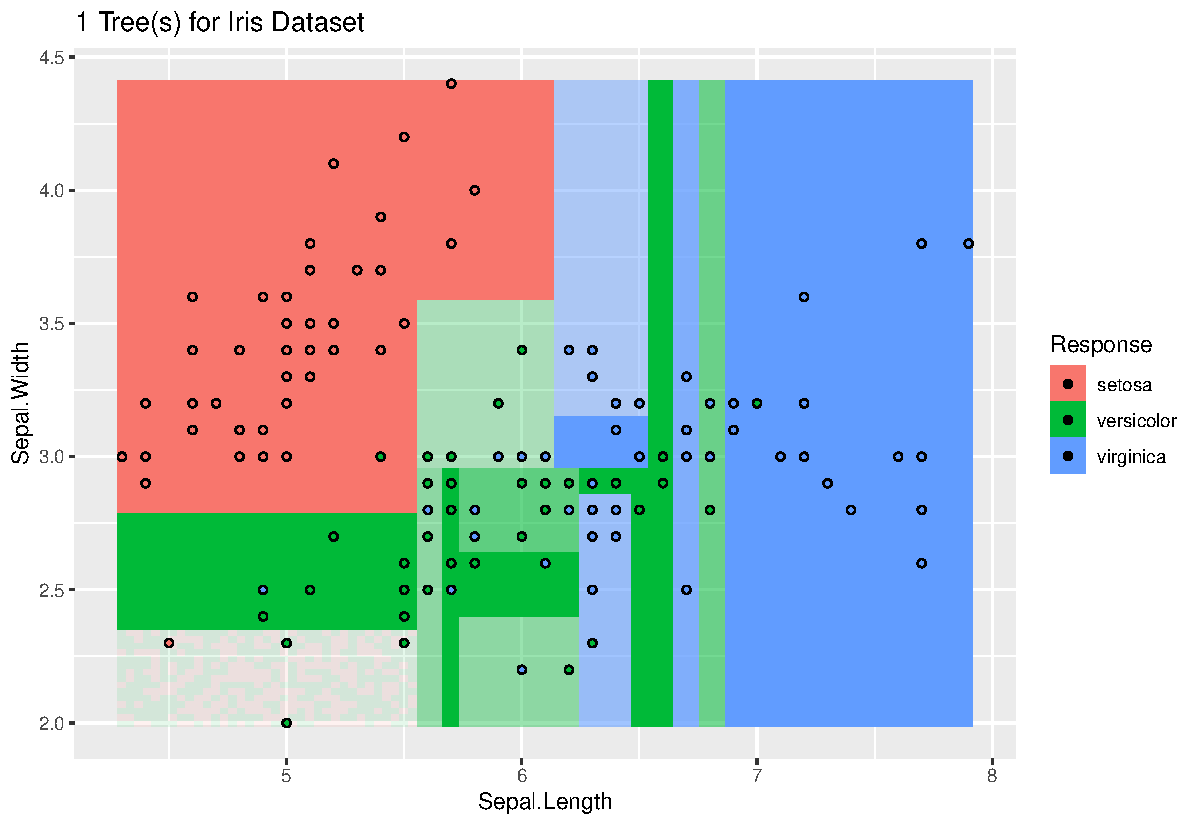
\includegraphics[width=0.95\textwidth]{figure/cart_forest_intro_1} 

}



\end{knitrout}
\begin{knitrout}\scriptsize
\definecolor{shadecolor}{rgb}{0.969, 0.969, 0.969}\color{fgcolor}

{\centering \includegraphics[width=0.95\textwidth]{figure/cart_forest_intro_2} 

}



\end{knitrout}
\begin{knitrout}\scriptsize
\definecolor{shadecolor}{rgb}{0.969, 0.969, 0.969}\color{fgcolor}

{\centering 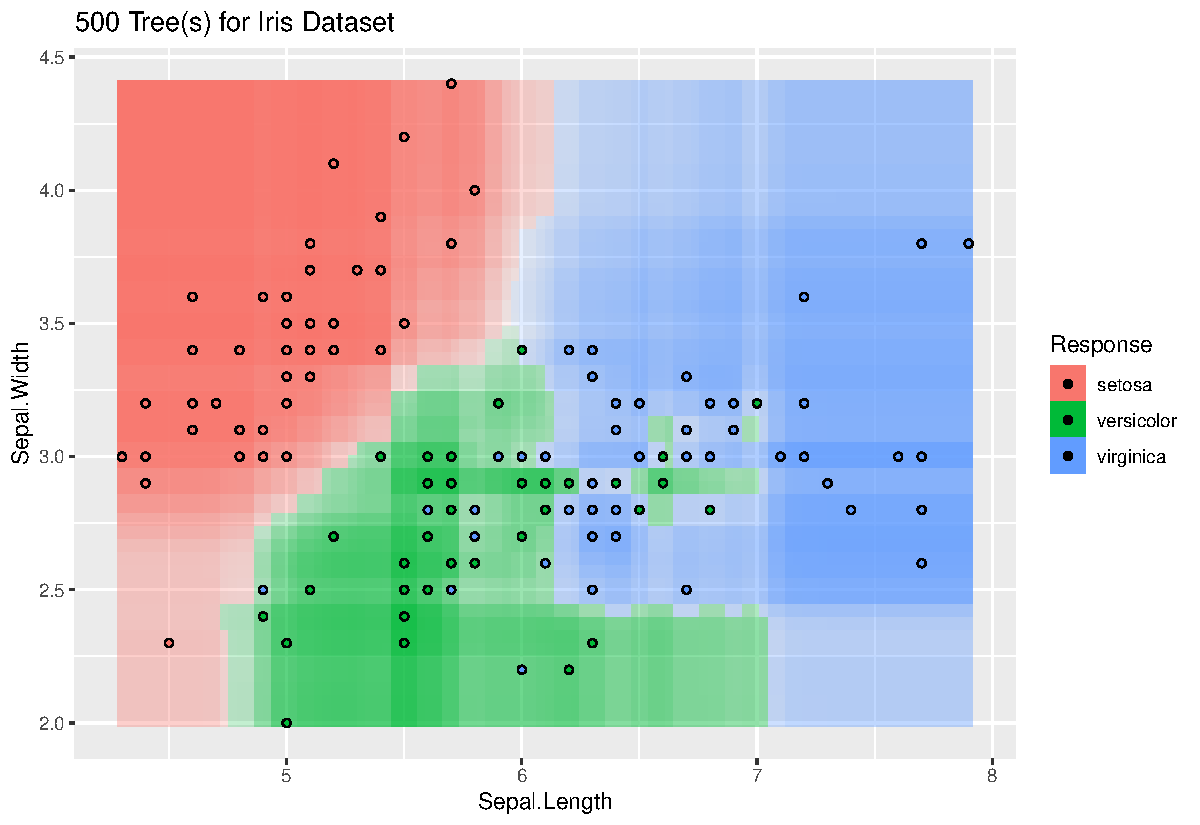
\includegraphics[width=0.95\textwidth]{figure/cart_forest_intro_3} 

}



\end{knitrout}
\end{vbframe}

\begin{vbframe}{Out-of-Bag Error Estimate}
With the RF it is possible to obtain unbiased estimates of the generalization error directly
during training, based on the out-of-bag observations for each tree:

\begin{knitrout}\scriptsize
\definecolor{shadecolor}{rgb}{0.969, 0.969, 0.969}\color{fgcolor}

{\centering \includegraphics[width=0.95\textwidth]{figure/cart_forest_intro_4} 

}



\end{knitrout}

\framebreak

\begin{center}
  % https://docs.google.com/drawings/d/1rxWgtVJEnurCPQ3njgDZ_JWPuQmiMfUttVU7q3Dr3Zs/edit
  \includegraphics[width=0.7\textwidth]{figure_man/forests-oob-error-2}
\end{center}

\footnotesize

\begin{itemize}
  \item For an estimation of the generalization error, we exploit the 
  fact that the $i$-th observation acts as unseen test point for all trees in 
  which it is OOB. 
  \item Let $\text{OOB}^{[m]}$ denote the index set 
  $\left \{i \in \setn | (\xv^{(i)}, \yi) \text{ is OOB for } \blm \right \}$.
  \item The number of trees for which the $i$-th observation is OOB is then 
  given by $S_{\text{OOB}}^{(i)} = 
  \sum_{m = 1}^M \I(i \in \text{OOB}^{[m]})$.
  \item We can compute the average over predictions $\hat{y}^{(i)[m]}$ from 
  trees $\blm$ that have observation $i$ in their OOB data to obtain an 
  ensemble prediction.
  \item The average loss of these ensemble OOB predictions over all $n$ 
  observations yields an estimate for the generalization error.
\end{itemize}
Compute the ensemble OOB prediction for each observation:
$$\yih_{\text{OOB}} = \begin{cases}
\frac{1}{S_{\text{OOB}}^{(i)}} \sum_{m = 1}^{M} 
\I(i \in \text{OOB}^{[m]}) \cdot \hat{y}^{(i)[m]}
& \text{in regression,} \\ 
\phantom{x} \\
\left[
\frac{1}{S_{\text{OOB}}^{(i)}} \sum_{m = 1}^{M} \I(i \in \text{OOB}^{[m]}) 
\cdot \I(\hat{h}^{(i)[m]} = k) \right]_{k \in \setg} &
\text{in classification.}
\end{cases}$$
\begin{itemize}
  \footnotesize
  \item This yields a scalar in regression and 
  a $g$-valued vector in classification.
  \item E.g., assume a classification task with $g = 3$ classes where 
  observation $i$ is OOB in $S_{\text{OOB}}^{(i)} = 10$ trees. If classes 1 to 
  3 are predicted 4, 4 and 2 times, respectively, we have 
  $\yih_{\text{OOB}} = (0.4, 0.4, 0.2)$.
  \item Eventually, take the average of the resulting point-wise losses to 
  estimate the OOB error of the forest:
  $$\widehat{\text{err}}_{\text{OOB}} = \meanin L(\yi, \yih_{\text{OOB}})$$
  \item OOB size: $\P(i \in \text{OOB}^{[m]}) = \left(1 - \frac{1}{n}\right)^n 
  \ \stackrel{n \to \infty}{\longrightarrow} \ \frac{1}{e} \approx 0.37$ for 
  $i \in \setn$.
  \item Similar to 3-CV, can be used for a quick model selection.
\end{itemize}

% \begin{itemize}
%   \item For an estimation of the generalization error, we exploit the 
%   fact that the $i$-th observation acts as unseen test point for all trees in 
%   which it is OOB. 
%   \item Let $\text{OOB}^{[m]}$ denote the index set 
%   $\left \{i \in \setn | (\xv^{(i)}, \yi) \text{ is OOB for } \blm \right \}$.
%   \item The number of trees for which the $i$-th observation is OOB is then 
%   given by $S_{\text{OOB}}^{(i)} = 
%   \sum_{m = 1}^M \I(i \in \text{OOB}^{[m]})$.
%   \item We can compute the average over predictions $\hat{y}^{(i)[m]}$ from 
%   trees $\blm$ that have observation $i$ in their OOB data to obtain an 
%   ensemble prediction.
%   \item The average loss of these ensemble OOB predictions over all $n$ 
%   observations yields an estimate for the generalization error.
%   \item Compute the ensemble OOB prediction for each observation:
%   $$\yih_{\text{OOB}} = \begin{cases}
%   \frac{1}{S_{\text{OOB}}^{(i)}} \sum_{m = 1}^{M} 
%   \I(i \in \text{OOB}^{[m]}) \cdot \hat{y}^{(i)[m]}
%   & \text{in regression,} 
%   \\ \phantom{x} \\
%   \left[
%   \frac{1}{S_{\text{OOB}}^{(i)}} \sum_{m = 1}^{M} \I(i \in \text{OOB}^{[m]}) 
%   \cdot \I(\hat{h}^{(i)[m]} = k) \right]_{k \in \setg} &
%   \text{in classification.}
%   \end{cases}$$
%   \begin{itemize}
%     \footnotesize
%     \item Note that the above formula yields a scalar regression and 
%     a $g$-valued probability vector in classification (with a 
%     slight abuse of notion, we might also predict a one-hot encoded class label 
%     in the latter case).
%     \item E.g., assume a classification task with $g = 3$ classes where 
%     observation $i$ is OOB in $S_{\text{OOB}}^{(i)} = 10$ trees. If classes 1 to 
%     3 are predicted 4, 4 and 2 times, respectively, we have 
%     $\yih_{\text{OOB}} = (0.4, 0.4, 0.2)$.
%   \end{itemize}
%   \item Eventually, take the average of the resulting point-wise losses to 
%   estimate the OOB error of the forest:
%   $$\widehat{\text{err}}_{\text{OOB}} = \meanin L(\yi, \yih_{\text{OOB}})$$
%   \item OOB size: $\P(i \in \text{OOB}^{[m]}) = \left(1 - \frac{1}{n}\right)^n 
%   \ \stackrel{n \to \infty}{\longrightarrow} \ \frac{1}{e} \approx 0.37$ for 
%   $i \in \setn$.
%   \item Similar to 3-CV, can be used for a quick model selection.
% \end{itemize}



\end{vbframe}

\endlecture
\end{document}
